\section{Gravitational Time Dilation}

In General Relativity, clocks deeper in a gravitational potential well run slower compared to those at higher potentials. We reproduce this result using æther flow fields instead of spacetime curvature.

\subsection*{Æther Flow as Gravity}

We assume that mass $M$ induces an inward radial flow of æther. At a radius $r$, this flow speed is given by:
\[
v_g(r) = \sqrt{\frac{2GM}{r}}.
\]

\begin{figure}[htbp]
    \centering
    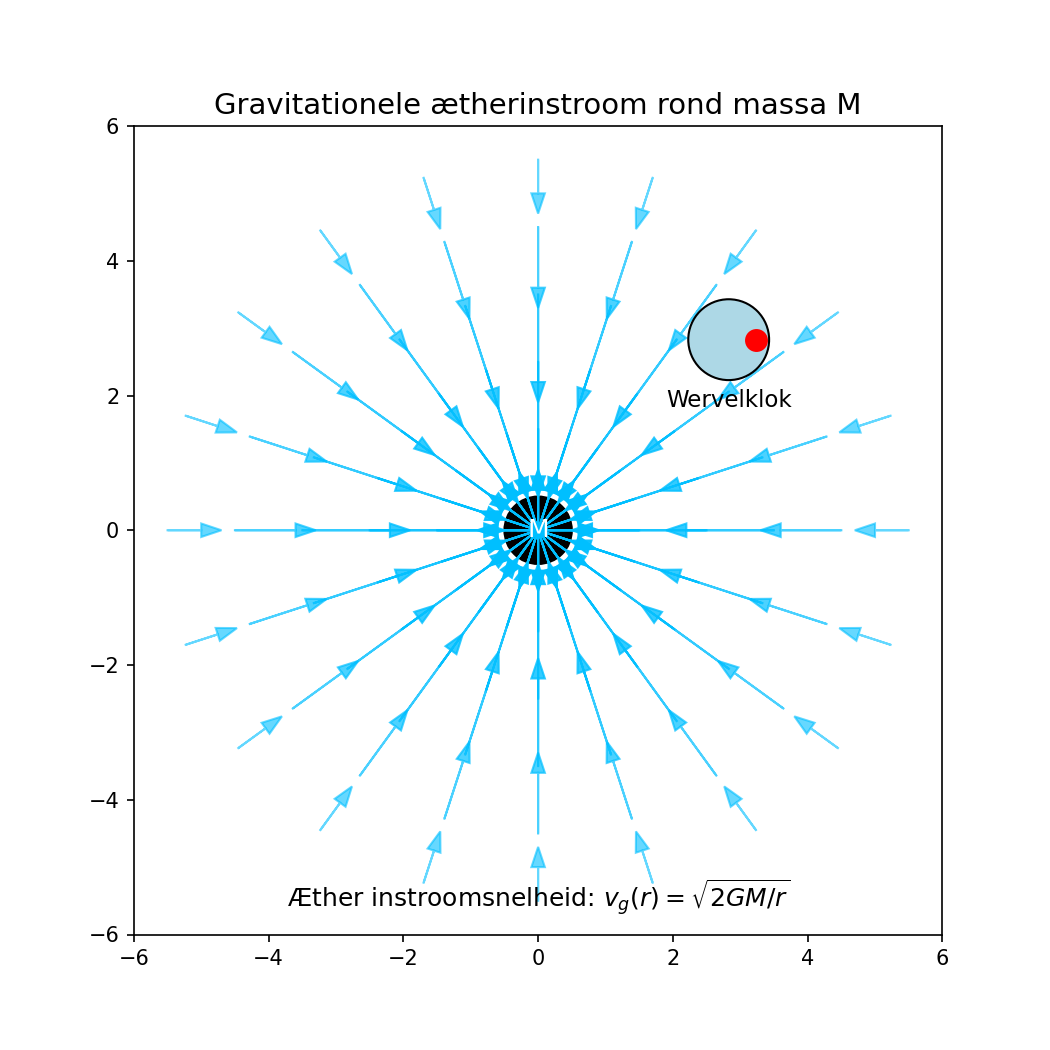
\includegraphics[width=0.85\textwidth]{images/07-GravitationeleÆtherinstroom}
    \caption{Gravitational time dilation due to radial æther inflow towards a mass~$M$. The vortex clock experiences a lower angular velocity due to æther drag, analogous to the Schwarzschild redshift.}
    \label{fig:GravitationeleÆtherinstroom}
\end{figure}

This mirrors the Painlevé–Gullstrand metric and the river model of black holes~\cite{Hamilton2004-river}.

\subsection*{Æther Drag and Clock Slowdown}

A clock held at radius $r$ in this inward æther flow sees æther moving past it at speed $v_g(r)$. The vortex core's observed angular velocity is therefore reduced due to the æther's drag, just as in the special relativity case, where motion through æther reduces the observed clock rate.

Thus, the gravitational time dilation factor is:
\[
\frac{d\tau}{dt} = \sqrt{1 - \frac{v_g^2(r)}{c^2}} = \sqrt{1 - \frac{2GM}{rc^2}}. \tag{4}
\]

A notable implication of gravitational æther inflow is related to the maximum force principle, defined as $F^{\text{gr}}_{\text{max}} = c^4 /4G$. Physically, this represents the upper limit on æther drag forces, where the inward æther flow near gravitational horizons reaches velocities close to ccc. At the Schwarzschild radius, the inflow speed of æther matches this limit, effectively freezing the rotation of any vortex-based clocks due to extreme drag, thus providing a tangible fluid-mechanical interpretation of gravitational horizons.

This is consistent with the Schwarzschild solution for stationary observers in general relativity.

A precise confirmation of gravitational time dilation under controlled conditions was provided by the Gravity Probe A mission~\cite{vessot_levine_1980}, which launched a hydrogen clock to an altitude of 10,000 km.

This delay was not only derived theoretically, but was confirmed experimentally by Pound and Rebka in 1959, who measured a gravitationally induced frequency shift between two points at different altitudes within the Earth's gravitational field using the Mössbauer effect~\cite{pound_rebka_1959}.

\subsection*{Interpretation}

This equation means that the deeper a vortex is located in the gravitational potential (the faster the local æther flow), the slower it rotates from the perspective of an observer at infinity. At the Schwarzschild radius $r_s = 2GM/c^2$, $d\tau/dt = 0$: time stops for external observers.

This provides a mechanistic interpretation of gravitational redshift: light emitted by a vortex-clock in a strong potential well appears redshifted due to the slower angular motion of the emitting vortex. The result:
\[
\boxed{\frac{d\tau}{dt} = \sqrt{1 - \frac{2GM}{rc^2}}}
\]
is fully consistent with GR and supports the æther flow analogy~\cite{Schiller2022-maxforce}.

\subsection*{Alternative Derivation via Æther Pressure Gradients}

An alternative and equally valid way to derive gravitational time dilation involves the use of Bernoulli\rqs s law for superfluids. Here, the gravitational potential is interpreted directly as a reduction in æther pressure near masses. According to Bernoulli\rqs s principle, a lower æther pressure corresponds to a higher local flow speed. Consequently, this pressure gradient interpretation aligns perfectly with the gravitational inflow velocity interpretation, providing theoretical versatility and enhancing the robustness of gravitational effects within the æther model.